\section{Data as Vectors and Matrices}

\begin{frame}{Observations, features and labels}
    \begin{center}
        \small
        \begin{tabular}{crrrr}
            \toprule
            & \multicolumn{3}{c}{features} & label \\
            \cmidrule(lr){2-4} \cmidrule(lr){5-5}
            $i$ & TV & radio & newspaper & sales \\
            \midrule
            1 & 230.1 & 37.8 & 69.2 & 22.1 \\
            2 & 44.5 & 39.3 & 45.1 & 10.4 \\
            $\vdots$ & $\vdots$ & $\vdots$ & $\vdots$ & $\vdots$ \\
            200 & 232.1 & 8.6 & 8.7 & 13.4 \\
            \bottomrule
        \end{tabular}
    \end{center}
    \begin{itemize}
        \item Each row is one \textbf{observation} (a market): $n = 200$ observations
        \item The columns TV, radio, newspaper are the \textbf{features} (predictors, inputs, independent variables): $p = 3$, budgets in thousands of dollars
        \item The column sales is the \textbf{label} (response, output, target, dependent variable): what we want to predict, in thousands of units
    \end{itemize}
\end{frame}

\begin{frame}{Vectors and matrices}
    \begin{itemize}
        \item Observation $i$ is a \textbf{feature vector} $\mathbf{x}^{(i)} = \big(x_1^{(i)}, x_2^{(i)}, \dots, x_p^{(i)}\big)^\top \in \mathbb{R}^p$ with label $y^{(i)} \in \mathbb{R}$; for example $\mathbf{x}^{(1)} = (230.1,\, 37.8,\, 69.2)^\top$ and $y^{(1)} = 22.1$
        \item Stacking the $n$ observations gives the \textbf{feature matrix} $\mathbf{X} \in \mathbb{R}^{n \times p}$, whose row $i$ is $(\mathbf{x}^{(i)})^\top$, and the \textbf{label vector} $\mathbf{y} \in \mathbb{R}^{n}$
    \end{itemize}
    \[
        \mathbf{X} = \begin{bmatrix} 230.1 & 37.8 & 69.2 \\ 44.5 & 39.3 & 45.1 \\ \vdots & \vdots & \vdots \\ 232.1 & 8.6 & 8.7 \end{bmatrix} = \begin{bmatrix} (\mathbf{x}^{(1)})^\top \\ (\mathbf{x}^{(2)})^\top \\ \vdots \\ (\mathbf{x}^{(n)})^\top \end{bmatrix}, \qquad \mathbf{y} = \begin{bmatrix} 22.1 \\ 10.4 \\ \vdots \\ 13.4 \end{bmatrix}
    \]
    \begin{itemize}
        \item Superscript $(i)$ = which observation (row), subscript $j$ = which feature (column): $x_j^{(i)}$ is entry $(i, j)$ of $\mathbf{X}$; bold lowercase = column vector, bold uppercase = matrix, plain letter = single number
    \end{itemize}
\end{frame}

\begin{frame}{The regression problem}
    \begin{itemize}
        \item Assume the label depends on the features through $y = f(\mathbf{x}) + \varepsilon$: $f$ is a fixed but unknown function and $\varepsilon$ is a random error with mean zero, independent of $\mathbf{x}$
        \item \textbf{Supervised learning}: estimate $f$ from the labelled data $\{(\mathbf{x}^{(i)}, y^{(i)})\}_{i=1}^{n}$, which gives an estimate $\hat{f}$
        \item \textbf{Regression} when the label is quantitative (sales, mpg, balance); classification when it is qualitative (later lectures)
        \item \textbf{Prediction}: compute $\hat{y} = \hat{f}(\mathbf{x})$ for new observations, treating $\hat{f}$ as a black box
        \item \textbf{Inference}: understand how the label changes with each feature (which features matter, how large the effects are, whether the relationship is linear)
    \end{itemize}
\end{frame}

\begin{frame}[allowframebreaks]{Advertising data: questions regression can answer}
    \begin{center}
        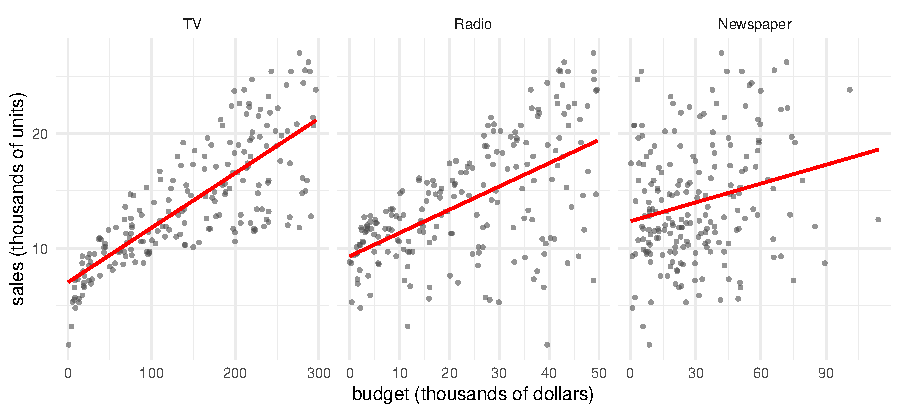
\includegraphics[width=0.95\linewidth,keepaspectratio]{figures/reg_advertising_scatter.pdf}
    \end{center}
    \begin{itemize}
        \item Is there a relationship between the advertising budgets and sales, and how strong is it?
        \item Which media are associated with sales, and by how much does each contribute?
        \item How accurately can we predict sales for given budgets?
        \item Is the relationship linear, and do the media reinforce each other (synergy)?
    \end{itemize}
\end{frame}

\section{Simple Linear Regression}

\begin{frame}{Simple linear regression model}
    \begin{itemize}
        \item One feature $x$ and a quantitative label $y$, related by a straight line plus error: $y = \beta_0 + \beta_1 x + \varepsilon$
        \item $\beta_0$ is the \textbf{intercept} (the value of $y$ when $x = 0$), $\beta_1$ is the \textbf{slope} (the change in $y$ for a one-unit increase in $x$); together they are the \textbf{coefficients}
        \item Estimate the coefficients from the training data (hat = estimated): $\hat\beta_0, \hat\beta_1$; predict with $\hat{y} = \hat\beta_0 + \hat\beta_1 x$
        \item \textbf{Fitted value} of observation $i$: $\hat{y}^{(i)} = \hat\beta_0 + \hat\beta_1 x^{(i)}$; \textbf{residual}: $e^{(i)} = y^{(i)} - \hat{y}^{(i)}$; residuals are computed from data, the errors $\varepsilon^{(i)}$ are never observed
        \item Example: $\text{sales} \approx \beta_0 + \beta_1 \times \text{TV}$
    \end{itemize}
\end{frame}

\begin{frame}[allowframebreaks]{Least squares criterion}
    \begin{center}
        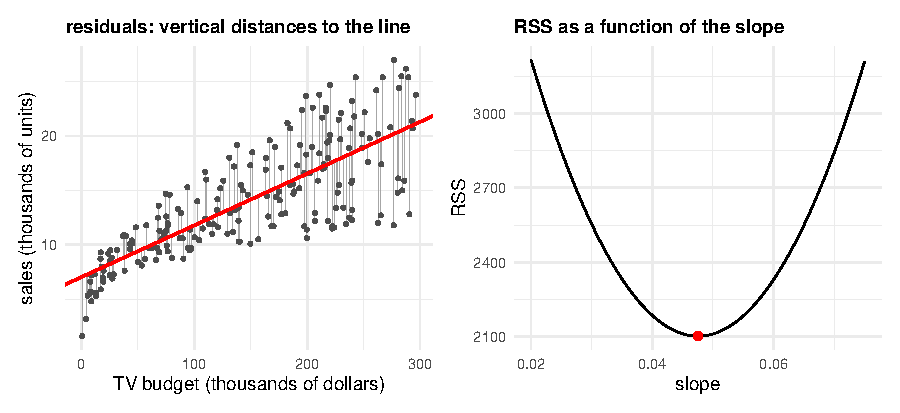
\includegraphics[width=0.95\linewidth,keepaspectratio]{figures/reg_slr_ls.pdf}
    \end{center}
    \begin{itemize}
        \item \textbf{Residual sum of squares}: $\mathrm{RSS} = \sum_{i=1}^{n} \big(e^{(i)}\big)^2 = \sum_{i=1}^{n} \big(y^{(i)} - \beta_0 - \beta_1 x^{(i)}\big)^2$
        \item \textbf{Least squares} chooses $\hat\beta_0, \hat\beta_1$ to minimize RSS: the line with the smallest total squared vertical distance to the points
        \item Squaring stops positive and negative residuals from cancelling and penalizes large ones more; the red dot marks the minimum (RSS $= 2102.5$ for TV)
    \end{itemize}
\end{frame}

\begin{frame}{Least squares estimates}
    Setting the partial derivatives of RSS with respect to $\beta_0$ and $\beta_1$ to zero gives closed-form estimates, where $\bar{x}$ and $\bar{y}$ are the sample means:
    \[
        \hat\beta_1 = \frac{\sum_{i=1}^{n} \big(x^{(i)} - \bar{x}\big)\big(y^{(i)} - \bar{y}\big)}{\sum_{i=1}^{n} \big(x^{(i)} - \bar{x}\big)^2}, \qquad \hat\beta_0 = \bar{y} - \hat\beta_1 \bar{x}
    \]
    \begin{itemize}
        \item $\hat\beta_1$ is the sample covariance of $x$ and $y$ divided by the sample variance of $x$
        \item The fitted line always passes through the point of means $(\bar{x}, \bar{y})$
        \item Advertising, sales on TV: $\hat\beta_0 = 7.03$ and $\hat\beta_1 = 0.0475$
    \end{itemize}
\end{frame}

\mode<article>{
    \paragraph{Derivation of the least squares estimates.}
    The partial derivatives of RSS are
    \begin{align*}
        \frac{\partial\, \mathrm{RSS}}{\partial \beta_0} &= -2 \sum_{i=1}^{n} \big(y^{(i)} - \beta_0 - \beta_1 x^{(i)}\big), &
        \frac{\partial\, \mathrm{RSS}}{\partial \beta_1} &= -2 \sum_{i=1}^{n} x^{(i)} \big(y^{(i)} - \beta_0 - \beta_1 x^{(i)}\big).
    \end{align*}
    Setting the first to zero gives $\bar{y} = \beta_0 + \beta_1 \bar{x}$, so $\hat\beta_0 = \bar{y} - \hat\beta_1 \bar{x}$. Substituting this into the second equation gives $\sum_i x^{(i)} (y^{(i)} - \bar{y}) = \hat\beta_1 \sum_i x^{(i)} (x^{(i)} - \bar{x})$, and since $\sum_i x^{(i)} (y^{(i)} - \bar{y}) = \sum_i (x^{(i)} - \bar{x})(y^{(i)} - \bar{y})$ and $\sum_i x^{(i)} (x^{(i)} - \bar{x}) = \sum_i (x^{(i)} - \bar{x})^2$, the formula for $\hat\beta_1$ follows.
}

\begin{frame}{Interpreting the coefficients}
    \begin{itemize}
        \item Fitted line for the Advertising data: $\widehat{\text{sales}} = 7.03 + 0.0475 \times \text{TV}$ (sales in thousands of units, TV budget in thousands of dollars)
        \item $\hat\beta_1 = 0.0475$: an additional \$1,000 of TV budget is associated with about $0.0475 \times 1000 = 47.5$ additional units sold
        \item $\hat\beta_0 = 7.03$: about 7,030 units are predicted when the TV budget is zero; the smallest TV budget in the data is \$700, so the intercept sits at the edge of the data
        \item The fit describes association in the observed markets; a causal reading needs more than a fitted line, because budgets were not assigned at random
    \end{itemize}
\end{frame}

\begin{frame}[allowframebreaks]{How accurate are the estimates?}
    \begin{center}
        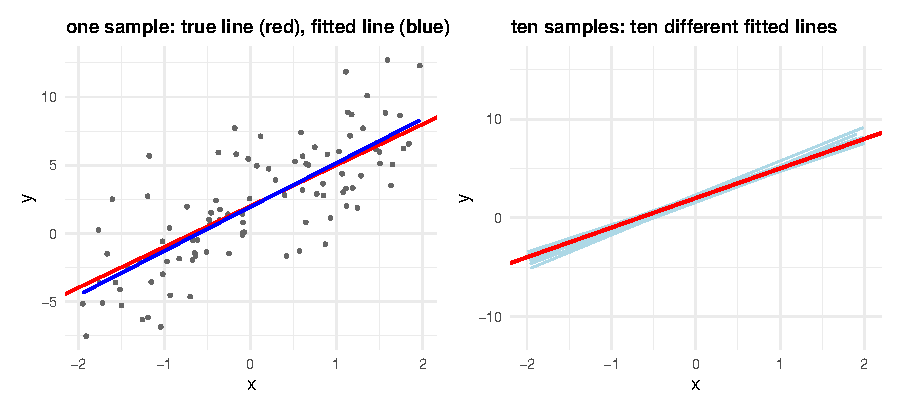
\includegraphics[width=0.95\linewidth,keepaspectratio]{figures/reg_slr_sampling.pdf}
    \end{center}
    \begin{itemize}
        \item The population regression line (red) is the true, unknown relationship; the least squares line (blue) is computed from one sample, and every new sample gives a different line
        \item On average the estimates are correct (unbiased), but a single $\hat\beta_1$ differs from $\beta_1$; the \textbf{standard error} measures the typical size of this difference
    \end{itemize}
\end{frame}

\begin{frame}{Standard errors of the coefficients}
    \[
        \mathrm{SE}(\hat\beta_1)^2 = \frac{\sigma^2}{\sum_{i=1}^{n} \big(x^{(i)} - \bar{x}\big)^2}, \qquad \mathrm{SE}(\hat\beta_0)^2 = \sigma^2 \bigg[\frac{1}{n} + \frac{\bar{x}^2}{\sum_{i=1}^{n} \big(x^{(i)} - \bar{x}\big)^2}\bigg]
    \]
    \begin{itemize}
        \item Here $\sigma^2 = \mathrm{Var}(\varepsilon)$ is the variance of the errors; standard errors shrink with more data, less noise, and more spread-out $x^{(i)}$
        \item $\sigma^2$ is unknown and is estimated from the residuals by $\mathrm{RSE}^2 = \mathrm{RSS}/(n-2)$; replacing $\sigma$ by RSE gives the estimated standard errors reported by software
        \item These formulas assume the errors are uncorrelated with constant variance $\sigma^2$ (checked with residual plots later)
        \item Advertising, sales on TV: $\mathrm{SE}(\hat\beta_0) = 0.4578$ and $\mathrm{SE}(\hat\beta_1) = 0.0027$
    \end{itemize}
\end{frame}

\begin{frame}{Confidence intervals and hypothesis tests (recap)}
    \begin{itemize}
        \item \textbf{95\% confidence interval} for $\beta_1$: approximately $\hat\beta_1 \pm 2 \cdot \mathrm{SE}(\hat\beta_1)$ (exactly, the $0.975$ quantile of the $t_{n-2}$ distribution replaces 2)
        \item \textbf{Hypothesis test}: $H_0\colon \beta_1 = 0$ (no relationship) against $H_a\colon \beta_1 \neq 0$, using $t = \hat\beta_1 / \mathrm{SE}(\hat\beta_1)$, which follows a $t_{n-2}$ distribution if $H_0$ is true
        \item The \textbf{$p$-value} is the probability of a $|t|$ at least this large if $H_0$ were true; a small $p$-value (say below 0.05) is evidence against $H_0$
        \item Advertising, sales on TV: 95\% confidence interval for $\beta_1$ is $[0.0422,\, 0.0528]$
    \end{itemize}
    \begin{center}
        \small
        \begin{tabular}{lrrrr}
            \toprule
            & coefficient & std. error & $t$-statistic & $p$-value \\
            \midrule
            intercept & 7.0326 & 0.4578 & 15.36 & $<0.0001$ \\
            TV & 0.0475 & 0.0027 & 17.67 & $<0.0001$ \\
            \bottomrule
        \end{tabular}
    \end{center}
\end{frame}

\begin{frame}{Assessing the fit: RSE and R-squared}
    \begin{itemize}
        \item \textbf{Residual standard error}: $\mathrm{RSE} = \sqrt{\mathrm{RSS}/(n-2)}$, the typical size of a residual, in the units of $y$; Advertising: $\mathrm{RSE} = 3.26$, about 3,260 units (23\% of the mean sales)
        \item \textbf{$R^2$}: the proportion of the variation in $y$ explained by the regression
    \end{itemize}
    \[
        R^2 = 1 - \frac{\mathrm{RSS}}{\mathrm{TSS}}, \qquad \mathrm{TSS} = \sum_{i=1}^{n} \big(y^{(i)} - \bar{y}\big)^2
    \]
    \begin{itemize}
        \item $0 \le R^2 \le 1$; Advertising: $R^2 = 1 - 2102.5/5417.2 = 0.612$, so TV explains about 61\% of the variance in sales
        \item In simple regression $R^2 = r^2$, the squared correlation between $x$ and $y$ ($r = 0.782$)
        \item RSE is in the units of $y$, $R^2$ is unit-free; a good $R^2$ depends on the application
    \end{itemize}
\end{frame}